\documentclass{article}
\usepackage[utf8]{inputenc}
\usepackage{amsmath}
\usepackage{amsthm}
\usepackage{xcolor}
\usepackage{authblk}
\usepackage{graphicx}
\usepackage{enumerate}
%\usepackage{enumitem}
\usepackage{mathrsfs}
\usepackage{amssymb}
\usepackage{caption}
\usepackage{subcaption}
\usepackage{float}
\usepackage{bbm}
\usepackage{geometry}
\usepackage{amsthm}
%\usepackage{subcaption}
\usepackage{istgame}
\usepackage{multirow,array}
\usepackage{sgame}


\title{QFM Exploration Notes}
\author{}
\date{\today}

\def\cei^#1_#2{\lower\fontdimen17\textfont2\vbox{%
   \baselineskip=\fontdimen17\textfont2 \advance\baselineskip by\fontdimen14\textfont2
   \halign{\hfil$\scriptstyle##$\hfil\cr#1\cr#2\cr}%
}}

\newcommand{\N}{\mathbb{N}}
\newcommand{\Z}{\mathbb{Z}}
\newcommand{\Ztilde}{\mathbf{\Tilde{Z}}}
\newcommand{\E}{\mathbb{E}}

\DeclareMathOperator*{\argmax}{\text{arg} \max}
\DeclareMathOperator*{\argmin}{\text{arg} \min}


\begin{document}

\newgeometry{left=1.0in,right=1.0in,top=1.0in,bottom=1.0in}
\maketitle

\section{Location-Scale Model Notes}

I consider the following DGP:

\begin{equation*}
	y_{it} = \alpha_i\beta_t + \eta_i\gamma_te_{it}
\end{equation*}

We require that $\eta_t\gamma_t > 0$, so we will draw them from the $\chi^2$ distribution. All together we have:

\[
	\alpha_i \sim \mathcal{N}(0, 1); \quad \beta_t \sim \mathcal{N}(0, 1); \quad \eta_i \sim \chi^2(1); \quad \gamma_t \sim \chi^2(1); \quad e_{it} \sim \mathcal{N}(0,1)
\]


Suppose $y_{it}$ is a scalar random variable, $\alpha_{i}, \beta_t, \gamma_t$, and $\eta_i$ are random vectors, and $e_{it}$ are i.i.d., in time and cross-section, and independent of $y, \alpha, \beta, \gamma,$ and $\eta_i$. Let $F$ be the cdf of $e_{it}$, and $Q(\tau )$ its $\tau $-th quantile. Suppose the DGP\ is

%
\begin{equation*}
	y_{it}= \alpha_i^{\prime }\beta_t +\eta_i^{\prime}\gamma_te_{it}.
\end{equation*}
%
Assume $\eta_i^{\prime}\gamma_t$ is always positive, then the conditional quantile function is

%
\begin{equation*}
	Q_{\tau }(y_{it}|\alpha_i, \beta_t, \eta_i ^{\prime}\gamma_t)=\alpha_i^{\prime}\beta_t + \eta_i^{\prime}\gamma_t F^{-1}(\tau)= \alpha_i^{\prime}\beta_t + \eta_i^{\prime}\gamma_t Q(\tau)
\end{equation*}
%

This is what the QPC algorithm estimates, and so with a two-factor model the factors estimated should*** span the same space as $\beta_t$ and $\gamma_t$. Then a regression the true $\gamma_t$ on $\hat{\beta}_t + \hat{\gamma}_t$ should have a high $R^2$. This is importantly only true if the estimated $\hat{\gamma}_t$ is actually converging to the true one. The estimated loadings should be an estimate of the true loading on the first factor $\hat{\alpha}_i$ and the $\tau$-th quantile of $F$. 

For simplicity, we will consider $e_{it} \sim \mathcal{N}(0, 1)$. Then for estimates at the median, we should expect that there is only one factor. For estimates at $\tau = 0.25$, we should expect that the mean value of the second estimated factor is  $\Phi^{-1}(0.25) = -0.67$.

We consider the DGP as above with $\alpha_i, \beta_t, w_i, x_t$ all i.i.d. $\mathcal{N}(0, 1)$. To satisfy $\eta_i^{\prime}\gamma_t > 0$, we define 

\begin{align*} 
	\eta_i  &= e^{w_i} \\
	\gamma_t &= e^{x_t} 
\end{align*}

We then generate data according to this DGP for $T = 1000, N = 100$. The average $R^2$ is reported in table \ref{table1}. 

\begin{figure}
	\centering
    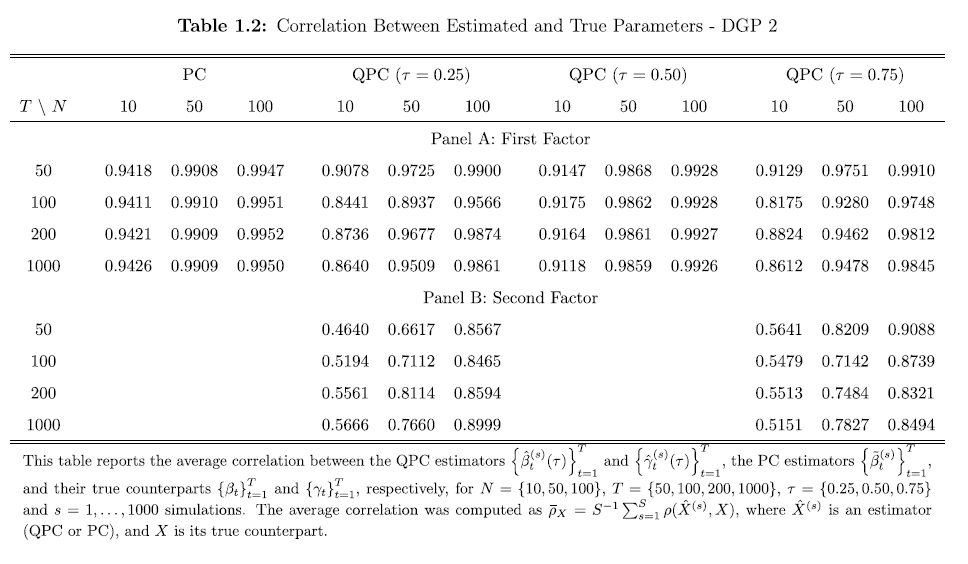
\includegraphics[width=0.9\linewidth]{../out/sagner_t2.png}
    \caption{Caption}
    \label{fig:enter-label}
\end{figure}


\end{document}






























